\chapter{Background}
	In this chapter a brief intruduction is given about the basic techniques used in this thesis.
	Section \ref{sec:background:SFS} gives a short description of the classic shape-from-shading problem and the basic assumptions. In section \ref{sec:background:CNN} a short introduction on convolutional neuronal networks  is given and how to make training deep neuronal network architectures more easy \ref{sec:background:mlCNN:resnet}.
	
%#########################################################
\section{Shape recovery using shading}
\label{sec:background:SFS}
	Three components are essential to the shape-from-shading (SFS) problem. The object whose shape should be estimated, the light source and the camera which produces the image of the surface  (see figure \ref{fig:surface_normal}). Considering a three-dimensional coordinate system $O(x,y,z)$ attached to the camera and $O(z)$  attached to the to the optical-axis then $O(x,y)$ coincides with the image plane:
	
	\begin{equation}
		\vec{x} = f \frac{x}{z}
		\quad \quad \quad  \quad 
		\vec{y} = f \frac{y}{z}
	\end{equation}
	
	where $(\vec{x},\vec{y})$ are the image coordinates of a point $(x,y,z)$ made by a camera with focal length $f$. 	
	As the image irradiance and the object irradiance are proportional, the shape-from-shading problem can then be formalized as the "image irradiance equation":
	
	\begin{equation}
	\label{eq:img_irradiance}
	R(p,q) = E(x,y)
	\end{equation}
	
	where $E(x,y)$ is the grayscale level (irradiance) of the image in point $(\vec{x},\vec{y})$ and $R(p,q)$ is the reflection function, giving the amount of re-emitted light from the surface depending on its orientation $(p,q)$. The orientation of a surface can be specified as by its gradient $(p,q,-1)$, where $p = \frac{\partial z}{\partial x}$ and $q = \frac{\partial z}{\partial y}$ are the first derivatives of z with respect to $x$ and $y$. So to derive the irradiance of an image knowledge about the light source ,camera and the objects reflection function is necessary. 
	With this set up the image irradiance equation can be used to analyze an images. So solving the first order non-linear partial differential equation in $\vec{x}$ and $\vec{y}$ will give the orientation $(p,y)$ and thus the shape of the surface. 
	\\ \\
	In view of the complexity of the SFS problem restrictions and assumptions have to be made. Therefore classic approaches assume a single point light source, a Lambertian (matt) surface and orthographic projection in order to make the problem solvable.	

	\begin{figure}
	 	\centering
	 	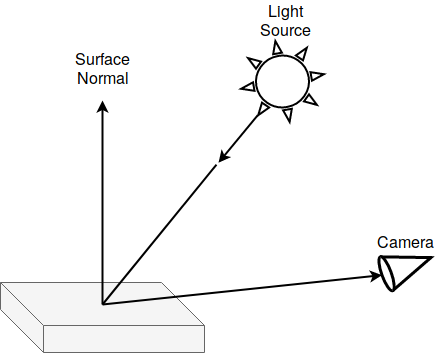
\includegraphics[height=0.2\textheight]{images/surface_normal.png}
	 	\caption{Image configuration for the shape-from-shading problem~\cite{Reflectance_map_techniques}.}
	 	\label{fig:surface_normal}
	\end{figure}
%#########################################################
	\subsection{Orthographic and perspective projection}
	\label{sec:background:projection}
	

%#########################################################
\section{Machine learning usinng CNN}
\label{sec:background:CNN}
- erklären wie CNN funktionieren? 
- Idee für encoder decoder Architektur erklären

%#########################################################
\subsection{Deep Residual Learning}
\label{sec:background:mlCNN:resnet}
	Deep residual neuronal networks 
	In view of the fact that deeper neuronal networks are harder to train
- erklären was ResNet ist \\
- wie funktionieren Residual
- Architektur von ResNet18
